
\documentclass[journal]{IEEEtran}
% *** CITATION PACKAGES ***
%
%\usepackage{cite}
% cite.sty was written by Donald Arseneau
% V1.6 and later of IEEEtran pre-defines the format of the cite.sty package
% \cite{} output to follow that of IEEE. Loading the cite package will
% result in citation numbers being automatically sorted and properly
% "compressed/ranged". e.g., [1], [9], [2], [7], [5], [6] without using
% cite.sty will become [1], [2], [5]--[7], [9] using cite.sty. cite.sty's
% \cite will automatically add leading space, if needed. Use cite.sty's
% noadjust option (cite.sty V3.8 and later) if you want to turn this off.
% cite.sty is already installed on most LaTeX systems. Be sure and use
% version 4.0 (2003-05-27) and later if using hyperref.sty. cite.sty does
% not currently provide for hyperlinked citations.
% The latest version can be obtained at:
% http://www.ctan.org/tex-archive/macros/latex/contrib/cite/
% The documentation is contained in the cite.sty file itself.



\usepackage[nodayofweek]{datetime}
\usepackage{todonotes}
\newcommand{\citeneeded}{\cite{NEEDED} \todo[color=green!40]{Citation needed}}

% *** GRAPHICS RELATED PACKAGES ***
%
\ifCLASSINFOpdf
  % \usepackage[pdftex]{graphicx}
  % declare the path(s) where your graphic files are
  % \graphicspath{{../pdf/}{../jpeg/}}
  % and their extensions so you won't have to specify these with
  % every instance of \includegraphics
  % \DeclareGraphicsExtensions{.pdf,.jpeg,.png}
\else
  % or other class option (dvipsone, dvipdf, if not using dvips). graphicx
  % will default to the driver specified in the system graphics.cfg if no
  % driver is specified.
  % \usepackage[dvips]{graphicx}
  % declare the path(s) where your graphic files are
  % \graphicspath{{../eps/}}
  % and their extensions so you won't have to specify these with
  % every instance of \includegraphics
  % \DeclareGraphicsExtensions{.eps}
\fi
% graphicx was written by David Carlisle and Sebastian Rahtz. It is
% required if you want graphics, photos, etc. graphicx.sty is already
% installed on most LaTeX systems. The latest version and documentation can
% be obtained at: 
% http://www.ctan.org/tex-archive/macros/latex/required/graphics/
% Another good source of documentation is "Using Imported Graphics in
% LaTeX2e" by Keith Reckdahl which can be found as epslatex.ps or
% epslatex.pdf at: http://www.ctan.org/tex-archive/info/
%
% latex, and pdflatex in dvi mode, support graphics in encapsulated
% postscript (.eps) format. pdflatex in pdf mode supports graphics
% in .pdf, .jpeg, .png and .mps (metapost) formats. Users should ensure
% that all non-photo figures use a vector format (.eps, .pdf, .mps) and
% not a bitmapped formats (.jpeg, .png). IEEE frowns on bitmapped formats
% which can result in "jaggedy"/blurry rendering of lines and letters as
% well as large increases in file sizes.
%
% You can find documentation about the pdfTeX application at:
% http://www.tug.org/applications/pdftex
\usepackage{graphicx}

% *** SUBFIGURE PACKAGES ***
%\usepackage[tight,footnotesize]{subfigure}
% subfigure.sty was written by Steven Douglas Cochran. This package makes it
% easy to put subfigures in your figures. e.g., "Figure 1a and 1b". For IEEE
% work, it is a good idea to load it with the tight package option to reduce
% the amount of white space around the subfigures. subfigure.sty is already
% installed on most LaTeX systems. The latest version and documentation can
% be obtained at:
% http://www.ctan.org/tex-archive/obsolete/macros/latex/contrib/subfigure/
% subfigure.sty has been superceeded by subfig.sty.



%\usepackage[caption=false]{caption}
%\usepackage[font=footnotesize]{subfig}
% subfig.sty, also written by Steven Douglas Cochran, is the modern
% replacement for subfigure.sty. However, subfig.sty requires and
% automatically loads Axel Sommerfeldt's caption.sty which will override
% IEEEtran.cls handling of captions and this will result in nonIEEE style
% figure/table captions. To prevent this problem, be sure and preload
% caption.sty with its "caption=false" package option. This is will preserve
% IEEEtran.cls handing of captions. Version 1.3 (2005/06/28) and later 
% (recommended due to many improvements over 1.2) of subfig.sty supports
% the caption=false option directly:
%\usepackage[caption=false,font=footnotesize]{subfig}
%
% The latest version and documentation can be obtained at:
% http://www.ctan.org/tex-archive/macros/latex/contrib/subfig/
% The latest version and documentation of caption.sty can be obtained at:
% http://www.ctan.org/tex-archive/macros/latex/contrib/caption/









% *** PDF, URL AND HYPERLINK PACKAGES ***
%
\usepackage{url}
% url.sty was written by Donald Arseneau. It provides better support for
% handling and breaking URLs. url.sty is already installed on most LaTeX
% systems. The latest version can be obtained at:
% http://www.ctan.org/tex-archive/macros/latex/contrib/misc/
% Read the url.sty source comments for usage information. Basically,
% \url{my_url_here}.


% correct bad hyphenation here
\hyphenation{op-tical net-works semi-conduc-tor}


\begin{document}
\title{COMP6033 - Individual Research Report}
%
%
% author names and IEEE memberships
% note positions of commas and nonbreaking spaces ( ~ ) LaTeX will not break
% a structure at a ~ so this keeps an author's name from being broken across
% two lines.
% use \thanks{} to gain access to the first footnote area
% a separate \thanks must be used for each paragraph as LaTeX2e's \thanks
% was not built to handle multiple paragraphs
%

\author{Henry Lovett}

% The paper headers
\markboth{Journal of \LaTeX\ Class Files,~Vol.~6, No.~1, January~2007}%
{Shell \MakeLowercase{\textit{et al.}}: Bare Demo of IEEEtran.cls for Journals}
% The only time the second header will appear is for the odd numbered pages
% after the title page when using the twoside option.
% 
% *** Note that you probably will NOT want to include the author's ***
% *** name in the headers of peer review papers.                   ***
% You can use \ifCLASSOPTIONpeerreview for conditional compilation here if
% you desire.


\maketitle


\begin{abstract}
%\boldmath
The abstract goes here.
\end{abstract}

\begin{IEEEkeywords}
IEEEtran, journal, \LaTeX, paper, template.
\end{IEEEkeywords}






% For peer review papers, you can put extra information on the cover
% page as needed:
% \ifCLASSOPTIONpeerreview
% \begin{center} \bfseries EDICS Category: 3-BBND \end{center}
% \fi
%
% For peerreview papers, this IEEEtran command inserts a page break and
% creates the second title. It will be ignored for other modes.
\IEEEpeerreviewmaketitle


%  Introduction.tex
%  Document created by seblovett on seblovett-Ubuntu
%  Date created: Wed 19 Feb 2014 09:02:42 GMT
%  <+Last Edited: Mon 17 Mar 2014 11:19:23 GMT by seblovett on seblovett-Ubuntu +>


\section{Introduction}
%\IEEEPARstart{L}{orem} Ipsum\dots\cite{chandrakasan1992low}.
\IEEEPARstart{T}{he} desire for low power devices has been driven by the mobile age.
Companies are competing on battery life of portable devices, such as smartphones and tablets.
This drive for low power has resulted in different synthesis techniques.
This paper will review and explore some of the techniques used to help reduce the power consumption of a circuit, with particular interest on the synthesis techniques used to do so.

%Two main branches of power - leakage and dynamic. 
%\inote{Explain these types of power}

There are two main categories of power consumption - dynamic and leakage. 
Dynamic power is the power consumed when the circuit is enabled and functioning. 
Power is used here through the charging and discharging of the internal capacitors of the module.
Leakage power is due to the non-ideal characteristics of sub-micron CMOS transistors.
Leakage power mainly occurs when the module is in a idle, non-switching state \cite{bsoul2010fpga} and can contribute around 22\% of the total power consumption of a $90nm$ FPGA \cite{altera2005}

The report begins with a review of different techniques in turn. 
This includes a brief introduction to the theory and a discussion of synthesis problems and solutions.
The report concludes by reviewing all techniques and their relevant advantages and disadvantages. 
%\inote{Define terms here.}


%%  PowerDomains.tex
%  Document created by seblovett on seblovett-NETBOOK
%  Date created: Wed 19 Feb 2014 11:26:11 GMT
%  <+Last Edited: Sat 22 Feb 2014 13:21:10 GMT by seblovett on seblovett-Ubuntu +>

\section{Power Domains}
This section reviews literature about Power Domains.


%  PowerDomains.tex
%  Document created by seblovett on seblovett-NETBOOK
%  Date created: Wed 19 Feb 2014 11:26:11 GMT
%  <+Last Edited: Tue 25 Mar 2014 18:49:57 GMT by seblovett on seblovett-Ubuntu +>

\section{Power Techniques}
\subsection{Power Gating}



Leakage currents begin to occur in sub-micron technologies, typically lower than 100nm \cite{bsoul2010fpga, nair2009comparative}.
With each technology generation, gate leakage increases 30 fold \cite{bernstein2003design}.
Leakage currents can are identified as two sources - sub-threshold currents and gate tunnelling. 
Sub-threshold currents occur when the voltage applied to the gate is lower than the transistor threshold voltage. 
The channel of the transistor during weak inversion still allows some current to flow from source to drain.
This current occurs when the transistor is off and is also exponentially dependant on $V_{th}$ \cite{borkar1999design}.
Gate tunnelling currents increase with thinner oxide layer \cite{m2002international}. 
A thin oxide results in electrons being able to pass through the gate into the substrate of the transistor. 
%This thin gate results in electrons passing through it, into the circuit causing leakage. 
Gate tunnelling occurs when the transistor is active \cite{nair2009comparative}.
Figure \ref{fig:leakage} shows where these leakage currents occur on an NMOS transistor.

\begin{figure}
\centering
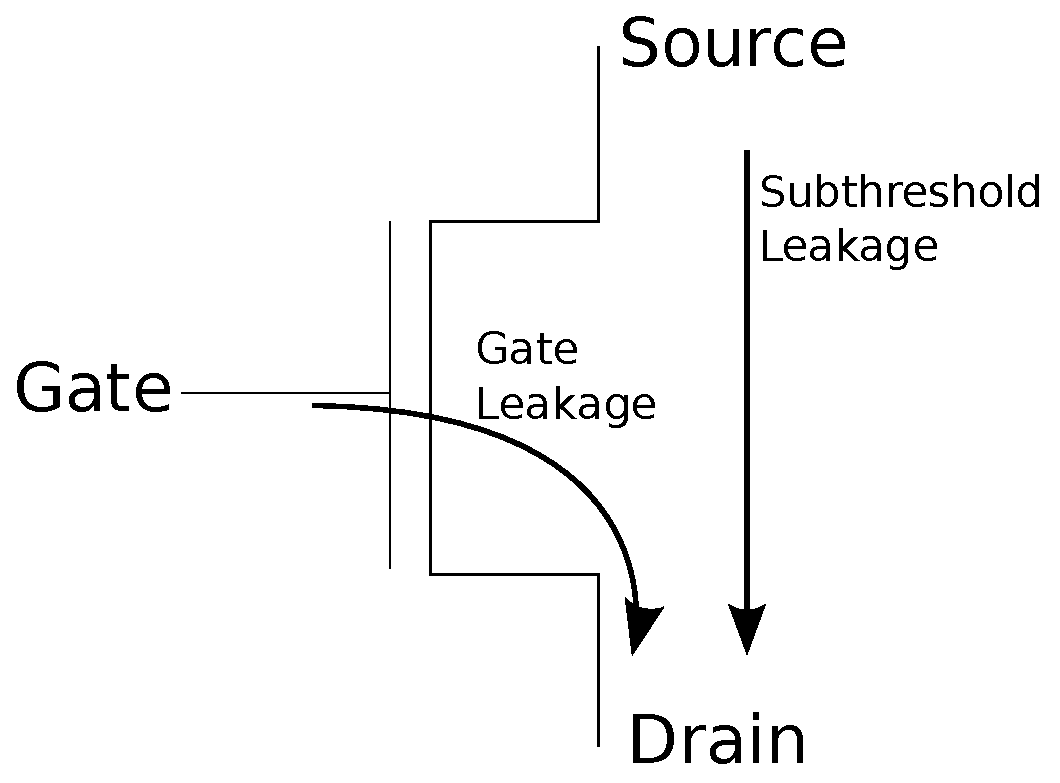
\includegraphics[width=0.4\textwidth]{Figures/leakage.eps}
\caption{The locations of gate and subthreshold leakage on an NMOS transistor}
\label{fig:leakage}
\end{figure}
%\todo[inline]{\cite{altera2005} has a good figure of the leakage currents}

\subsubsection{Theory}

Power gating, in principle, is where the power to a module is switched off when not in use. 
By doing this, the module does not consume any power. 
It can be achieved by using either a header or a footer switch to disable either the supply connection or the ground connection. 
Figure \ref{fig:powerswitches} shows the realisation of the power gating circuits.

\begin{figure}[h]
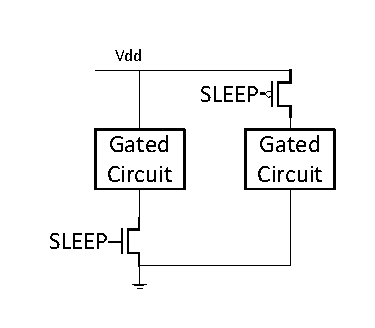
\includegraphics[width=0.5\textwidth]{Figures/powergating_switches.pdf}
\caption{Circuit diagrams showing the use of footer switches (left) or header switches (right).}
\todo[inline]{Break this into two subfigures}
\label{fig:powerswitches}
\end{figure}

Although the theory of operation is simple, the technique poses many issues in the implementation.
Firstly, as the module is floating, the outputs are undefined.
This can cause the gates in another module to short circuit - at an input voltage of $ V_{dd} / 2 $, both the NMOS and PMOS transistors will be on, resulting in a direct line from supply to ground. 
The solution to this is is to add logic gates with a `clamp' signal. 
This could be either an \texttt{AND} gate, of which the clamp signal is active low, or an \texttt{OR} gate with an active high clamp. 
This added logic is needed per output signal of the power gated module.

The second issue that power gating raises is when the gated module contains sequential logic. 
By removing the power to the sequential logic, the state is lost. 
This can then cause issues as state retention may be necessary, as well as low power.
The solution is to use a state retention register. 
There is a timing overhead involved to store the register before putting the device to sleep, disabling the majority of the circuit. 
State retention registers also require an ungated power supply, meaning all power gated modules require two supplies; one which is gated and one constant supply.

The final aspect of power gating that needs addressing is the power management.
The power manager is responsible for when to gate the module.% on and off.
As well as the control of the sleep transistors, the power manager is also responsible for the stopping the clock, clamping the outputs and saving the state to the state retention mechanism.

There is a large overhead in the additional circuitry needed for power gating. 
The main increase are the state retention registers as these can require 20\% more area in silicon \cite{stateretarea}. 
Other techniques exist to avoid this, such as the use of the scan path to quickly clock the state in and out to/from memory.
Digital signal processing, however, would not need this as it is data dependent. 
Processors with cache have a large amount of state data, so state retention registers are needed here.

When footer switches are used, the voltage that at the source of the NMOS is known as the virtual ground (VGND). When the footer is active, VGND $\approx$ GND. When off, VGND $\approx V_{dd}$.
A full realisation of a power gated circuit is shown in figure \ref{fig:powergated}. 


\begin{figure}
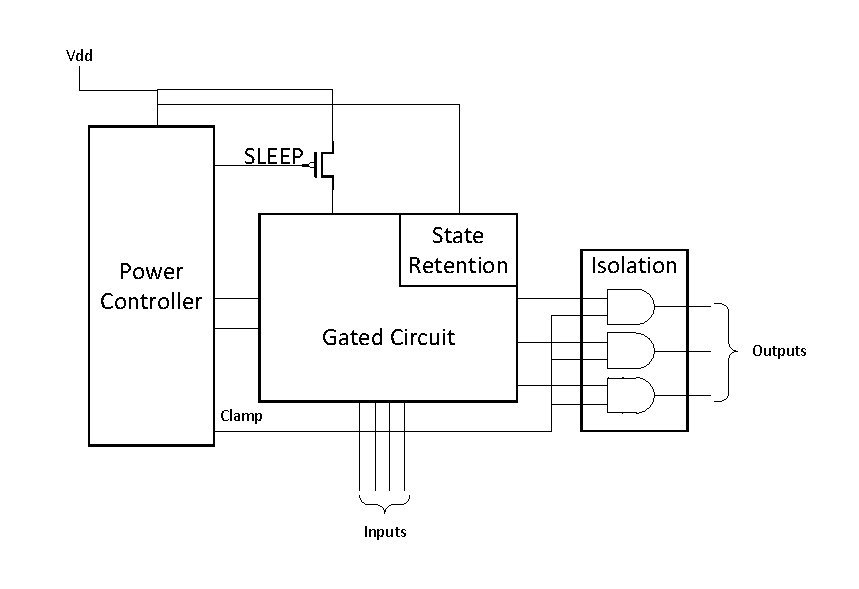
\includegraphics[width=0.5\textwidth]{Figures/powergating_full.pdf}
\caption{The realisation of a power gated module. State retention, isolation and a power manager are all needed}
\label{fig:powergated}
\end{figure}


\subsubsection{Synthesis Techniques}

%Fine and coarse grain techniques
Power gating can be split into two techniques, fine and coarse grain.
Fine grain gating is where individual cells (e.g. in ASIC) have their own gating transistor. 
Coarse grain techniques are where gating transistors are applied on a larger module scale.
\cite{nair2009comparative} compares the fine grain and coarse grain methods on a 65nm FPGA technology. 
Here, a SRAM block is used as the test circuit. 
Fine grain, in this case, is where the memory of each cell is individually gated, and coarse is where a $16 \times 1$ SRAM module is gated. 
It was conclusively shown that coarse grain gating reduced power consumption more than fine grain due to being able to turn off the read/write circuitry. 


%Multi sleep mode
When deciding to sleep a module, there are a number of overheads.
Due to the charging / discharging of the gated circuit (depending on the use of header or footer switches), when the circuit is re-enabled, there is an amount of time needed to allow the capacitors to return to normal \cite{abdollahi2005effective}.
This is referred to as the wake-up time and can also include the time to restore state if applicable.
The (dis)charging can also poses ground bounce issues to the device due to the sudden draw of current, \cite{kim2003understanding,chang1997analysis}. 

This wake up time can then impact the performance of the device - if more energy is consumed waiting for the disabled module than it would have consumed being awake, the overall power is not reduced.
\cite{kim2004experimental} discusses a method where an intermediate power saving mode is introduced.
This is done by using a standard footer power gating NMOS. 
An extra PMOS is then added in parallel with the power gating switch. 
Table \ref{tab:kim} summarises the states of the transistors in the circuit in figure \ref{fig:kim}

The RUN and COLD states operate as previously discussed. 
The PARK state, however, is where the virtual ground voltage does not rise to $V_{dd}$ due to the PMOS conducting. 
The virtual ground is at the threshold voltage of the PMOS, so the leakage current is less than in the RUN state, but not so high that state retention is needed. 
This drastically reduces the wake up overhead of the circuit. 

\begin{figure}
\centering
%\missingfigure{\cite{kim2004experimental} power states circuit}
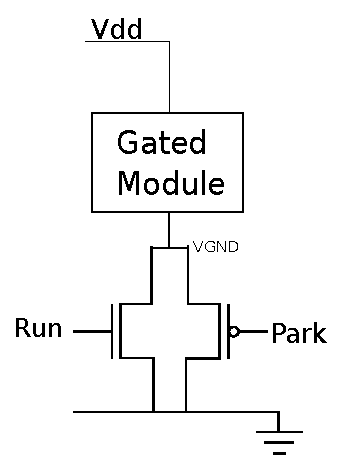
\includegraphics{Figures/powergating_kim.eps}
\caption{Middle power state implementation used in \cite{kim2004experimental}}
\label{fig:kim}
\end{figure}

\begin{table}
\caption{Power saving modes of \cite{kim2004experimental}}
\label{tab:kim}
\centering
\begin{tabular}{|c|c|c|c|}\hline
State Name & NMOS State & PMOS State & Virtual Ground Voltage (V)\\ \hline
RUN  & ON   & OFF  & GND \\
COLD & OFF  & OFF  & $V_{DD}$ \\
PARK & OFF  & ON   & $V_{th}$ PMOS \\ \hline
\end{tabular}
\end{table}

A further improvement to this single extra state is proposed in \cite{singh2007enhanced}. 
Here, multiple intermediate power states are implemented by using different sub-threshold gate voltages on the NMOS footer switch. 
The compromise of wake up time against leakage reduction can then be more finely controlled to best suit the circuit.
In general, the closer the virtual ground is to ground, the more leakage current occurs, but a faster wake up is available. 

\subsection{Power Scaling}

\inote{I want to try and find use of two modules, one with a Low $V_t$ for high performance, high power, and a high $V_t$ for low performance, low power, which can be switched between. 
If not, just look at multi $V_t$ technologies}
%\inote{What actually am I wanting to discuss here?}
\inote{Or I could look into adaptive body bias?}

\subsubsection{Theory}


\subsubsection{Synthesis Techniques}

%  FrequencyDomains.tex
%  Document created by seblovett on seblovett-NETBOOK
%  Date created: Wed 19 Feb 2014 11:28:09 GMT
%  <+Last Edited: Sat 22 Mar 2014 14:40:20 GMT by seblovett on seblovett-Ubuntu +>


\subsection{Frequency Domains}
Lowerm Ipson\dots

%%  PowerScaling.tex
%  Document created by seblovett on seblovett-NETBOOK
%  Date created: Wed 19 Feb 2014 11:28:42 GMT
%  <+Last Edited: Sat 22 Feb 2014 13:21:22 GMT by seblovett on seblovett-Ubuntu +>


\section{Power Scaling}
Lorem Ipsum\dots


%  FrequencyScaling.tex
%  Document created by seblovett on seblovett-NETBOOK
%  Date created: Wed 19 Feb 2014 11:29:26 GMT
%  <+Last Edited: Sat 22 Feb 2014 13:20:56 GMT by seblovett on seblovett-Ubuntu +>

\section{Frequency Scaling}
Lorem Ipsum\dots


%  ClockGating.tex
%  Document created by seblovett on seblovett-Ubuntu
%  Date created: Sat 22 Feb 2014 13:20:20 GMT
%  <+Last Edited: Sat 22 Mar 2014 14:40:49 GMT by seblovett on seblovett-Ubuntu +>

\subsection{Clock Gating}

\subsubsection{Theory}

The clock in a sequential circuit can consume 15-45\% of the power \cite{pedram1996power}.
Therefore it is a large area of potential power saving.
Clock gating is an approach of controlling the clock to individual modules of a design by either stopping or slowing down the clock with respect to a master clock \cite{841927}. 
An approach, seen in \cite{tellez1995activity}, involves stopping the clock to unused modules.

This method can be realised using two simple circuits seen in figures \ref{fig:cg:circuit1} and \ref{fig:cg:circuit2}.
Although figure \ref{fig:cg:circuit1} is functionally complete, in reality, a latch is needed to remove any glitches in the circuit.
These are fundamentally different to load-enable registers, where the input is multiplexed between the current value or the input.
The load-enable registers are still clocked at the master clock frequency.

\begin{figure}
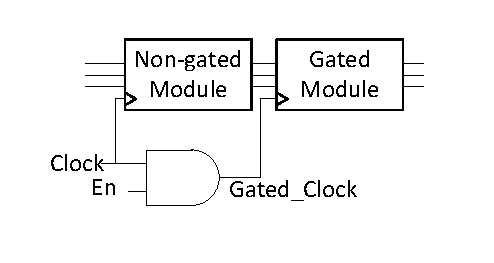
\includegraphics[width=0.5\textwidth]{Figures/clockgating_and.pdf}
\caption{Clock gating circuit using an \texttt{AND} gate}
\todo[inline]{Gated Module or Gated Circuit? Consistency with the other diagrams}
\todo[inline]{Is this even needed?}
\label{fig:cg:circuit1}
\end{figure}

\begin{figure}
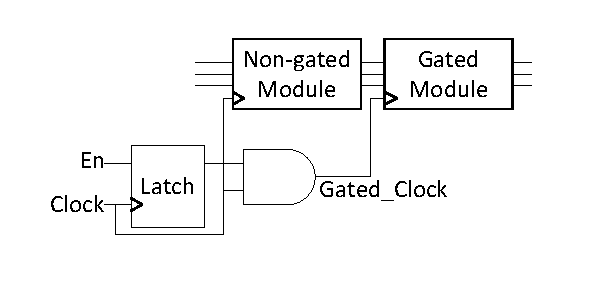
\includegraphics[width=0.5\textwidth]{Figures/clockgating_latch.pdf}
\caption{Clock gating circuit using an \texttt{AND} gate and a latch}
\todo[inline]{Gated Module or Gated Circuit? Consistency with the other diagrams}
\label{fig:cg:circuit2}
\end{figure}

\subsubsection{Synthesis Techniques}

A gating function is typically defined by the designer within the RTL design stage.
However, a more common approach is to allow the synthesis tool to obtain the gating functions from a gate-level netlist \cite{benini1999symbolic, hurst2008automatic}.

The general outline for the synthesis is to find the clock gating function for each flip-flop.
The flip-flops are then grouped so that they are driven by the same function. 
The problem of simplifying the gating function is looked at in \cite{han2012synthesis}. 
Here, an algorithm is suggested where the gating function is shared by existing combinational logic.
This was shown to reduce the logic added by introducing clock gating.

However, sometimes the addition of clock gating is not advantageous. 
The gating function can be large and therefore can cause timing violations, resulting in an unsuitable synthesis.
If the gating function is large enough, it can also consume more power than it saves.
Both of these issues are addressed in \cite{arbel2009resurrecting}.
Here, the author proposed solutions to large gating functions by reducing the depth of logic by an approximation. 
The approximation is made such that the resulting logic does not gate the clock more than the original function. 
It results in the flip-flop being clocked more often, but reduces the logic so that it can be utilised, thereby saving some power.
\cite{arbel2009resurrecting} also proposes the use of a clustering algorithm that looks at grouping similar gating functions. 
This can then reduce the overall logic needed to implement the clock gating and maximise the energy saved.

\subsubsection{Conclusion}

Clock gating is a simple principle to implement on a small scale.
The underlying theory is to disable a module when it is not in use.
This is done by identifying a gating function which disallows clock propagation if the function is asserted.

However, clock gating can produce large gating functions which violate the timing constraints of the circuit, or even consume more power than they save. This results in two problems that need solving - group formation and simplification \cite{han2012synthesis, paik2012clock}.








%\section{Introduction}
% The very first letter is a 2 line initial drop letter followed
% by the rest of the first word in caps.
% 
% form to use if the first word consists of a single letter:
% \IEEEPARstart{A}{demo} file is ....
% 
%\IEEEPARstart{T}{his} demo file is intended to serve as a ``starter file''
%for IEEE journal papers produced under \LaTeX\ using
%IEEEtran.cls version 1.7 and later.
% You must have at least 2 lines in the paragraph with the drop letter
% (should never be an issue)
%I wish you the best of success.

\hfill mds
 
\hfill \today

%\subsection{Subsection Heading Here}
%Subsection text here.

% needed in second column of first page if using \IEEEpubid
%\IEEEpubidadjcol

%\subsubsection{Subsubsection Heading Here}
%Subsubsection text here.


% An example of a floating figure using the graphicx package.
% Note that \label must occur AFTER (or within) \caption.
% For figures, \caption should occur after the \includegraphics.
% Note that IEEEtran v1.7 and later has special internal code that
% is designed to preserve the operation of \label within \caption
% even when the captionsoff option is in effect. However, because
% of issues like this, it may be the safest practice to put all your
% \label just after \caption rather than within \caption{}.
%
% Reminder: the "draftcls" or "draftclsnofoot", not "draft", class
% option should be used if it is desired that the figures are to be
% displayed while in draft mode.
%
%\begin{figure}[!t]
%\centering
%\includegraphics[width=2.5in]{myfigure}
% where an .eps filename suffix will be assumed under latex, 
% and a .pdf suffix will be assumed for pdflatex; or what has been declared
% via \DeclareGraphicsExtensions.
%\caption{Simulation Results}
%\label{fig_sim}
%\end{figure}

% Note that IEEE typically puts floats only at the top, even when this
% results in a large percentage of a column being occupied by floats.


% An example of a double column floating figure using two subfigures.
% (The subfig.sty package must be loaded for this to work.)
% The subfigure \label commands are set within each subfloat command, the
% \label for the overall figure must come after \caption.
% \hfil must be used as a separator to get equal spacing.
% The subfigure.sty package works much the same way, except \subfigure is
% used instead of \subfloat.
%
%\begin{figure*}[!t]
%\centerline{\subfloat[Case I]\includegraphics[width=2.5in]{subfigcase1}%
%\label{fig_first_case}}
%\hfil
%\subfloat[Case II]{\includegraphics[width=2.5in]{subfigcase2}%
%\label{fig_second_case}}}
%\caption{Simulation results}
%\label{fig_sim}
%\end{figure*}
%
% Note that often IEEE papers with subfigures do not employ subfigure
% captions (using the optional argument to \subfloat), but instead will
% reference/describe all of them (a), (b), etc., within the main caption.


% An example of a floating table. Note that, for IEEE style tables, the 
% \caption command should come BEFORE the table. Table text will default to
% \footnotesize as IEEE normally uses this smaller font for tables.
% The \label must come after \caption as always.
%
%\begin{table}[!t]
%% increase table row spacing, adjust to taste
%\renewcommand{\arraystretch}{1.3}
% if using array.sty, it might be a good idea to tweak the value of
% \extrarowheight as needed to properly center the text within the cells
%\caption{An Example of a Table}
%\label{table_example}
%\centering
%% Some packages, such as MDW tools, offer better commands for making tables
%% than the plain LaTeX2e tabular which is used here.
%\begin{tabular}{|c||c|}
%\hline
%One & Two\\
%\hline
%Three & Four\\
%\hline
%\end{tabular}
%\end{table}


% Note that IEEE does not put floats in the very first column - or typically
% anywhere on the first page for that matter. Also, in-text middle ("here")
% positioning is not used. Most IEEE journals use top floats exclusively.
% Note that, LaTeX2e, unlike IEEE journals, places footnotes above bottom
% floats. This can be corrected via the \fnbelowfloat command of the
% stfloats package.



%\section{Conclusion}
%The conclusion goes here.





% if have a single appendix:
%\appendix[Proof of the Zonklar Equations]
% or
%\appendix  % for no appendix heading
% do not use \section anymore after \appendix, only \section*
% is possibly needed

% use appendices with more than one appendix
% then use \section to start each appendix
% you must declare a \section before using any
% \subsection or using \label (\appendices by itself
% starts a section numbered zero.)
%


\appendices
%\section{Proof of the First Zonklar Equation}
%Appendix one text goes here.

% you can choose not to have a title for an appendix
% if you want by leaving the argument blank
%\section{}
%Appendix two text goes here.


% use section* for acknowledgement
%\section*{Acknowledgment}


%The authors would like to thank...


% Can use something like this to put references on a page
% by themselves when using endfloat and the captionsoff option.
\ifCLASSOPTIONcaptionsoff
  \newpage
\fi



% trigger a \newpage just before the given reference
% number - used to balance the columns on the last page
% adjust value as needed - may need to be readjusted if
% the document is modified later
%\IEEEtriggeratref{8}
% The "triggered" command can be changed if desired:
%\IEEEtriggercmd{\enlargethispage{-5in}}

% references section

% can use a bibliography generated by BibTeX as a .bbl file
% BibTeX documentation can be easily obtained at:
% http://www.ctan.org/tex-archive/biblio/bibtex/contrib/doc/
% The IEEEtran BibTeX style support page is at:
% http://www.michaelshell.org/tex/ieeetran/bibtex/
\bibliographystyle{IEEEtran}
% argument is your BibTeX string definitions and bibliography database(s)
\bibliography{bibliography}
%
% <OR> manually copy in the resultant .bbl file
% set second argument of \begin to the number of references
% (used to reserve space for the reference number labels box)
%\begin{thebibliography}{1}
%
%\bibitem{IEEEhowto:kopka}
%H.~Kopka and P.~W. Daly, \emph{A Guide to \LaTeX}, 3rd~ed.\hskip 1em plus
%  0.5em minus 0.4em\relax Harlow, England: Addison-Wesley, 1999.
%
%\end{thebibliography}

% biography section
% 
% If you have an EPS/PDF photo (graphicx package needed) extra braces are
% needed around the contents of the optional argument to biography to prevent
% the LaTeX parser from getting confused when it sees the complicated
% \includegraphics command within an optional argument. (You could create
% your own custom macro containing the \includegraphics command to make things
% simpler here.)
%\begin{biography}[{\includegraphics[width=1in,height=1.25in,clip,keepaspectratio]{mshell}}]{Michael Shell}
% or if you just want to reserve a space for a photo:

%\begin{IEEEbiography}{Michael Shell}
%Biography text here.
%\end{IEEEbiography}
%
%% if you will not have a photo at all:
%\begin{IEEEbiographynophoto}{John Doe}
%Biography text here.
%\end{IEEEbiographynophoto}

% insert where needed to balance the two columns on the last page with
% biographies
%\newpage

\begin{IEEEbiographynophoto}{Henry Lovett}
Henry is a fourth year MEng Student at the University of Southampton.
\end{IEEEbiographynophoto}

% You can push biographies down or up by placing
% a \vfill before or after them. The appropriate
% use of \vfill depends on what kind of text is
% on the last page and whether or not the columns
% are being equalized.

%\vfill

% Can be used to pull up biographies so that the bottom of the last one
% is flush with the other column.
%\enlargethispage{-5in}



% that's all folks
\end{document}


